% !TeX root = skripta-konstitutivni-vztahy.tex
% !TeX lastmodified = 2018-12-11

\subsection{Model porušení Bai-Wierzbicki}\label{sec:bai-wierzbicki}
Model\footnote{Bai Y. , Wierzbicki T.:  A new model of metal plasticity and fracture with pressure and Lode dependence. International Journal of Plasticity, 2008, vol. 24, pp. 1071-1096.} popisuje přesněji závislost porušení na deformačně napěťovém stavu, ale nezahrnuje vliv teploty a~rychlosti deformace. Kumulaci poškození popisuje opět parametr poškození počítaný integrálem
\begin{equation}
	D = \int\limits_0^{\bar{\varepsilon}_p} \frac{\diff \bar{\varepsilon}_p}{\bar{\varepsilon}_f(\eta, \bar{\theta})},
\end{equation}
kde lomové přetvoření $\bar{\varepsilon}_f$ je funkcí triaxiality napětí $\eta$ a~normalizovaného Lodeho úhlu $\bar{\theta}$.

Model pro ně zavádí následující tvar:
\begin{equation}\begin{split}
	\bar{\varepsilon}_f(\eta, \bar{\theta})
	= \big\{&\tfrac{1}{2} \left[ N_1 \exp(-N_2 \eta) + N_5 \exp(-N_6 \eta) \right] - N_3 \exp(-N_4 \eta) \big\} \bar{\theta}^2\\
	+ &\tfrac{1}{2} \left[ N_1 \exp(-N_2 \eta) - N_5 \exp(-N_6 \eta) \right] \bar{\theta} + N_3 \exp(-N_4 \eta)
\end{split}\end{equation}
kde $N_1$, $N_2$, $N_3$, $N_4$, $N_5$ a~$N_6$ jsou bezrozměrné parametry modelu.

Porušení nastane, když parametr poškození dosáhne jednotkové hodnoty ($D=1$).

\begin{figure}[H]
	\label{fig:typy-napjatosti-kalibracnich-teles}
	\centering
	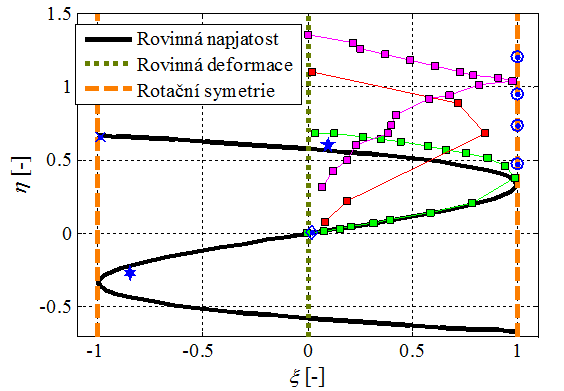
\includegraphics[width=0.7\textwidth]{typy-napjatosti-kalibracnich-teles}
	\caption[Typy napjatostí kalibračních těles]{Typy napjatostí kalibračních těles v~prostoru Lodeho parametr -- součinitel triaxiality napětí}
\end{figure}

\subsubsection{Kalibrační tělesa modelů plasticity a~porušení}
Tahová zkouška vzorku s~vrubem umožňuje měnit jen součinitel triaxiality.

Složitější vzorky:
\begin{itemize}
	\item Plech se dvěma symetrickými vruby v~tahu a~smyku
	\item Zkouška rovnoměrným dvouosým tahem (ekvibiaxiální)
	\item Pěchování válcových vzorků
	\item Trubka se dvěma ostrými vruby zevnitř a~zvenku
\end{itemize}

\begin{figure}[H]
	\label{fig:kalibracni-telesa-modelu-plasticity}
	\centering
	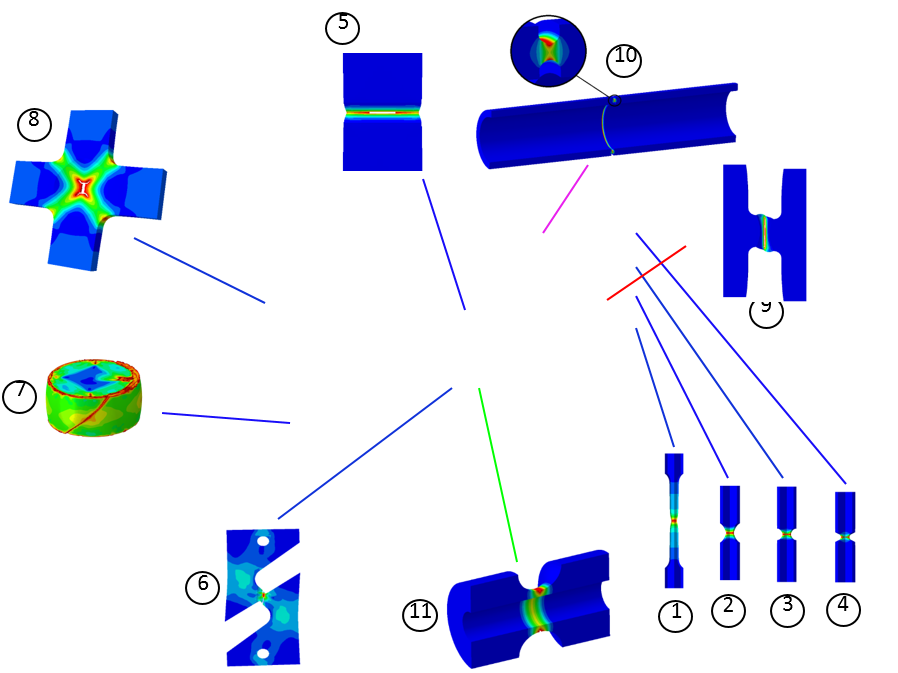
\includegraphics[width=0.6\linewidth]{kalibracni-telesa-modelu-plasticity}
	\caption{Kalibrační tělesa modelů}
\end{figure}

Lomové přetvoření lze zobrazit v~prostoru s~osami $\eta-\bar{\theta}-\bar{\varepsilon}_f$.
\begin{figure}[H]
	\label{fig:lomove-pretvoreni}
	\centering
	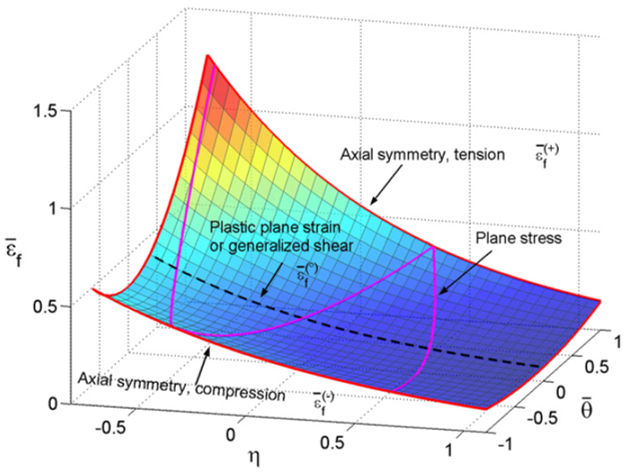
\includegraphics[width=0.7\linewidth]{lomove-pretvoreni}
	\caption{Grafická interpretace modelu}
\end{figure}
